
We now run DPC and MPC controller in a closed-loop simulation with the HAMLab plant model. 
The objective function and the box constraints on input and states are exactly same in both cases. Only difference in the optimization problem is due to system dynamics. In particular, MPC solves \eqref{E:mpc},  DPC-RT solves \eqref{E:dpcrt} and DPC-En \eqref{E:dpcrf}. $\mathsf{T}_{\mathrm{ref}}$ in the optimization problems is set to $18\,\mathrm{^oC}$. 


\subsection{Simulation Settings}
We test the performance of DPC controller against MPC controller on June 1, 2000. The choice of this day is arbitrary, and does not fall in the training period. For the HAMLab simulation model under consideration, the hourly weather predictions are only available from 1971-2000, however, the choice of the year does not influence the comparison. 
Heat gain due to occupancy $\mathsf{Q}_{\mathrm{oc}}$ is discrete variable which is defined to be $500\,\mathrm{W}$ from $8\,\mathrm{am}$ to $6\,\mathrm{pm}$ and $0\,\mathrm{W}$ otherwise. The disturbances on June 1, 2000 are shown in Fig.~\ref{F:dist}. The sampling time $T_s$ in MPC and model training for DPC is $5\,\mathrm{min}$, while the weather data is available after every $1\,\mathrm{h}$, so these disturbances are kept constant for 12 time steps. 
$N$ and $\delta$ are again chosen to be $6$. For solving optimization numerically, we use Gurobi Optimizer \cite{Gurobi2015}.

\subsection{Results}

Optimal control strategies for all 3 methods are shown in Fig.~\ref{F:control}. The chosen reference temperature and external disturbances require both heating and cooling at some point during the day. The solution obtained from MPC sets the benchmark that we compare to. 
Note that the MPC implementation uses the exact knowledge of the plant dynamics. Therefore, the associated control strategy is indeed the optimal strategy for the plant.
In reality the quality of data, and modeling errors also affect the performance of the MPC controller~\cite{behl2014model}.
Qualitatively, the DPC-En control input is not much different from that of MPC. Until $8\,\mathrm{am}$, when the disturbances are not changing to a great extent, MPC and DPC-En are very close. Slightly after $8\,\mathrm{am}$, when solar heat, external temperature and heat due to occupancy all increase abruptly, we observe that DPC-En cools less and differs slightly from the benchmark. Although DPC-RT also maintains the trend in the control input when the disturbances increase or decrease, the control strategy is quite different from that of MPC. Due to high variance in the predictions, DPC-RT also results in non-smooth inputs, which are not good for practical reasons of switching constraints on heating and cooling equipment in buildings.

\begin{figure}[t!]
\centering
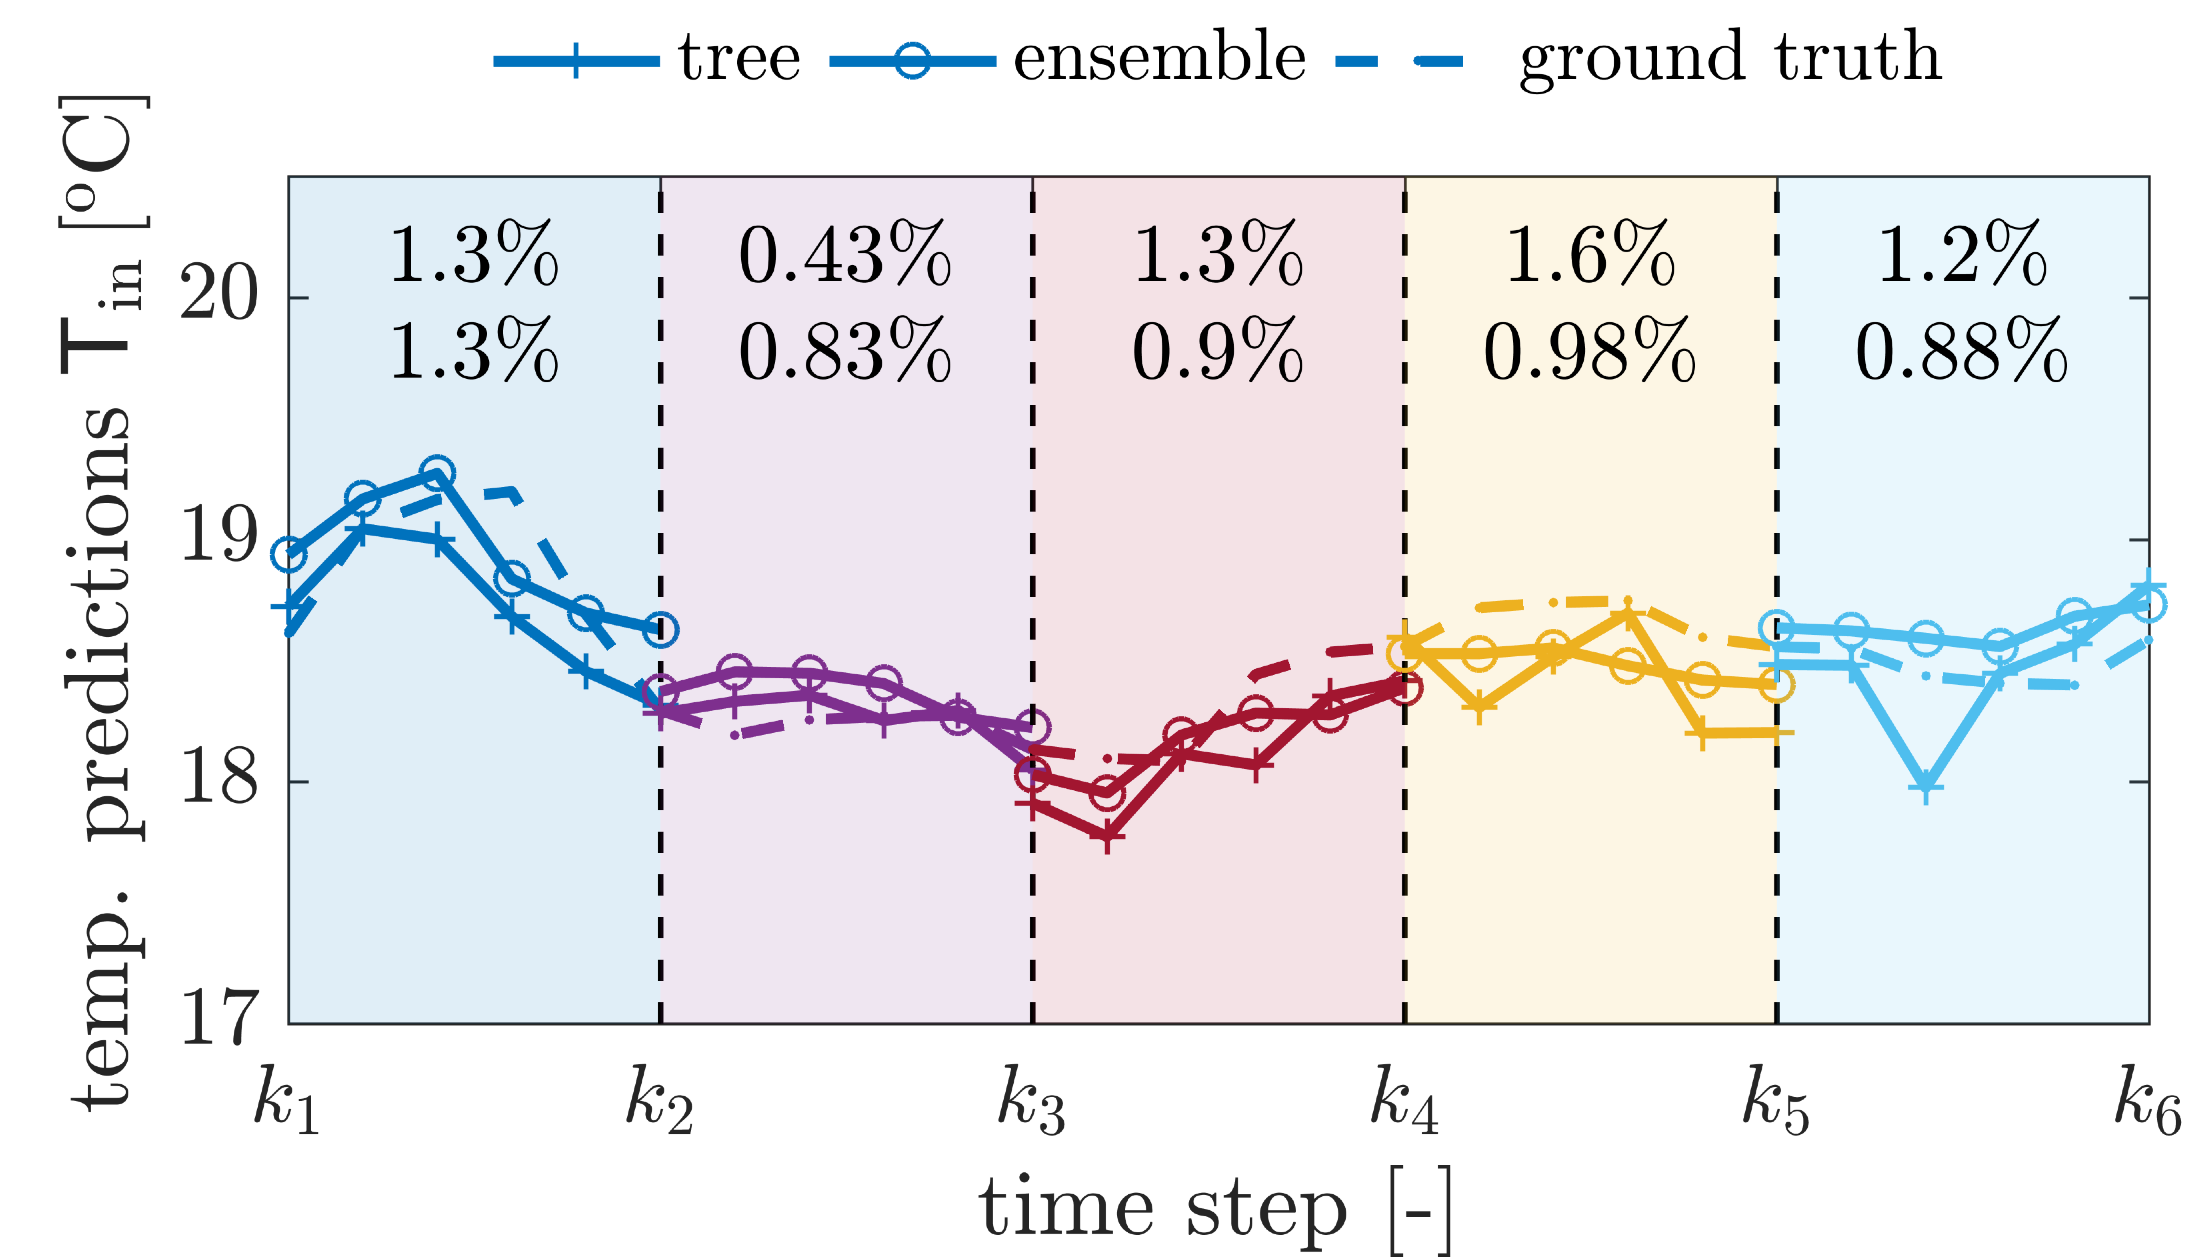
\includegraphics[width=21pc]{figures/pred_hzn.eps}
\caption{Accuracy of predictions with snapshots in time: at time $k_1$, we make 6 predictions for time $k_1$ to $k_1+5$. The numbers represent mean accuracy in predictions for these steps for trees (top) and ensembles (bottom). This process is repeated at time $k_2, \ldots, k_5$.}
\captionsetup{justification=centering}
\label{F:pred_accuracy}
\end{figure}
\begin{figure}[t!]
\centering
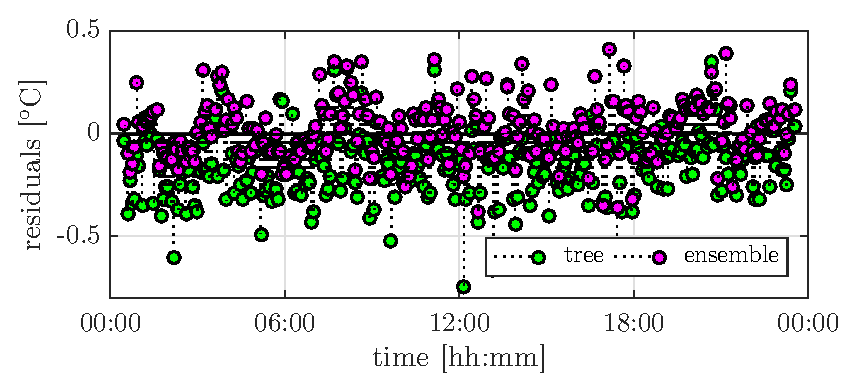
\includegraphics[width=21pc]{figures/residual.eps}
\caption{Residual error $\mathsf{T}_{\mathrm{pred}} - \mathsf{T}_{\mathrm{act}}$ for the tree $\mathcal{T}_{1}$  and the forest $\mathcal{R}_1$ that predict $\mathsf{T}_{\mathrm{in,k+1}}$ shows that the residuals for the forest are more concentrated around 0, while tree predictions have a much higher variance.}
\captionsetup{justification=centering}
\label{F:residuals}
\end{figure}
Fig.~\ref{F:state} shows the plot for the zone air temperature. Again, DPC-RT shows a bigger deviation from the optimal solution while DPC-En is near-optimal. This is attributed to linear model averaging in ensemble learning which improves the model prediction. This improvement comes at the cost of reduced interpretability.

\begin{figure}[t!]
\subfigure[Hourly weather data $\mathsf{T}_{\mathrm{ex}}$ and $\mathsf{Q}_{\mathrm{sl}}$ and internal disturbance $\mathsf{Q}_{\mathrm{in}}$.]{
\label{F:dist}
\centering
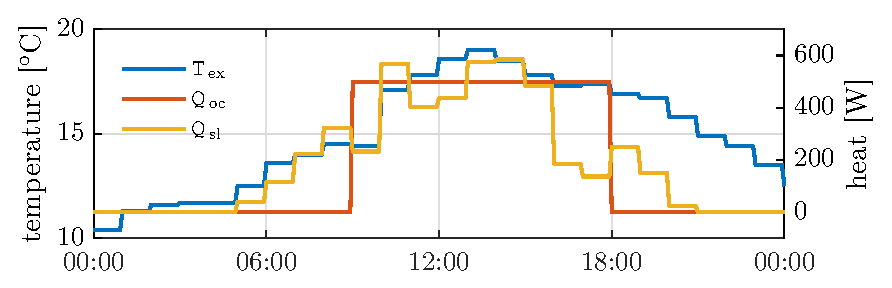
\includegraphics[width=21pc]{figures/dist.eps}
}
\subfigure[Optimal control strategies $\mathsf{Q}_{\mathrm{in}}$.]{
\label{F:control}
\centering
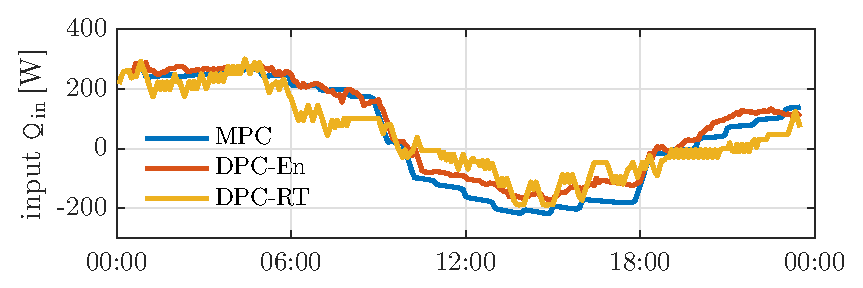
\includegraphics[width=21pc]{figures/control.eps}
}
\subfigure[Optimal internal zone air temperature $\mathsf{T}_{\mathrm{in}}$.]{
\label{F:state}
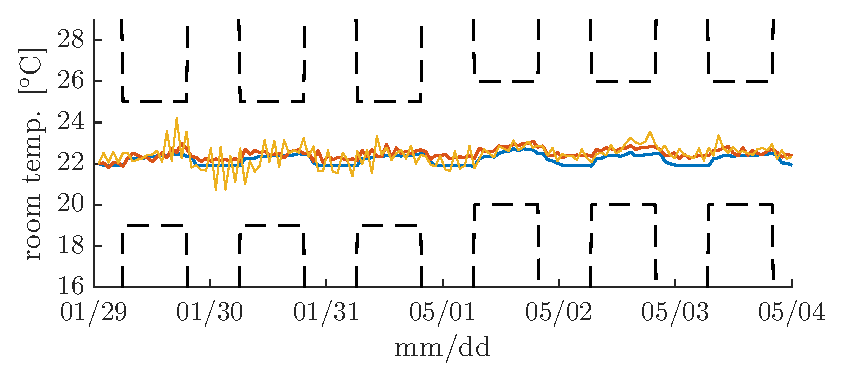
\includegraphics[width=21pc]{figures/state.eps}
}
\subfigure[Cumulative sum of the objective function.]{
\label{F:obj}
\centering
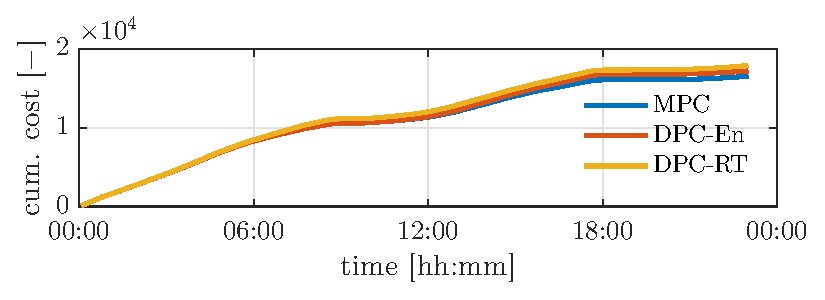
\includegraphics[width=21pc]{figures/obj.eps}
}
%\vspace{-1cm}
\caption{Comparison of optimal performance obtained with MPC, DPCRT and DPC-En on June 1, 2000. All 3 controllers start from the same state of the model.}
\captionsetup{justification=centering}
\end{figure}
The quantitative results from the simulations are tabulated in Tab.~\ref{T:quant}. We are interested in evaluating how close DPC performs in comparison to optimal benchmark set by MPC. The coefficient of determination or the $R^2$ score shows that 95.3\% variability in MPC has been accounted for by DPC-En, while DPC-RT captures only 83.9\% variability. In other words, DPC-En and MPC control inputs are 95.3\% close. Fig.~\ref{F:obj} shows the cumulative sum of the objective function as a function of time. At the end of the day, the cumulative sum for DPC-En is 3.8\% more than MPC, and for DPC-RT it is 8.1\% more than MPC. While both DPC-En and DPC-RT are near-optimal, the value of the objective function validates that DPC-En is more closer to the optimal solution.
In the considered scenario, MPC tracks the reference temperature more closely offering better thermal comfort than DPC-RT or DPC-En by spending more energy.